%!TEX TS-program = xelatex
%!TEX encoding = UTF-8 Unicode

\documentclass[11pt,tikz,border=1]{standalone}
\usepackage{graphicx}
\usepackage[default,mdseries=Light,bfseries=Medium,path=fonts]{cjkfonts}
\usetikzlibrary{calc,positioning,arrows.meta,shapes.geometric,shapes.misc }

\begin{document}
  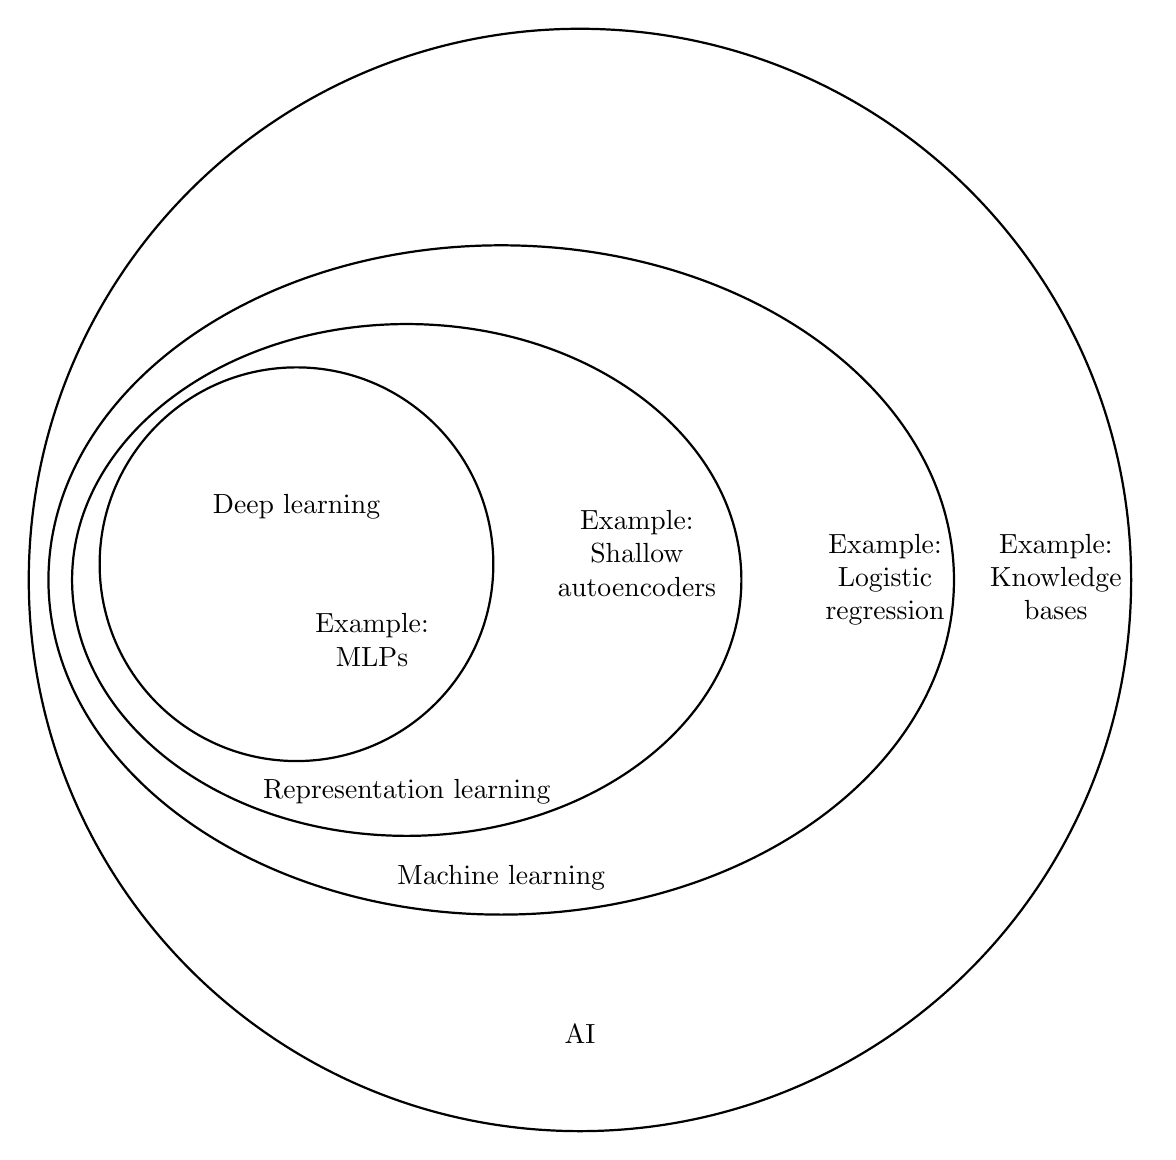
\begin{tikzpicture}[
    bigcycle/.style={circle,draw,thick,inner sep=0pt,minimum size=14cm},
    bigellipse/.style={shape=ellipse,draw,thick,minimum width=11.5cm,minimum height=8.5cm},
    smallellipse/.style={shape=ellipse,draw,thick,minimum width=8.5cm,minimum height=6.5cm},
    smallcycle/.style={circle,draw,thick,inner sep=0pt,minimum size=5cm}
    ]
    
    \node(ai) [bigcycle] {};
    \node(ai_title) [above=10mm] at (ai.south) {AI};
    \node(ai_ex) [left,xshift=2mm] at (ai.east) {
      \begin{tabular}{c}
        Example:\\
        Knowledge\\
        bases\\
      \end{tabular}
    };
    
    \node(ml) [bigellipse,xshift=-1cm] {};
    \node(ml_title) [above=2mm] at (ml.south) {Machine learning};
    \node(ml_ex) [left,xshift=2mm] at (ml.east) {
      \begin{tabular}{c}
        Example:\\
        Logistic\\
        regression\\
      \end{tabular}
    };
    
    \node(rl) [smallellipse,xshift=-2.2cm] {};
    \node(rl_title) [above=3mm] at (rl.south) {Representation learning};
    \node(rl_ex) [left,yshift=3mm] at (rl.east) {
      \begin{tabular}{c}
        Example:\\
        Shallow\\
        autoencoders\\
      \end{tabular}
    };
    
    \node(dl) [smallcycle,xshift=-3.6cm,yshift=2mm] {};
    \node(dl_title) [below=1.5cm] at (dl.north) {Deep learning};
    \node(dl_ex) [left,xshift=-5mm,yshift=-10mm] at (dl.east) {
      \begin{tabular}{c}
        Example:\\
        MLPs\\
      \end{tabular}
    };
    
  \end{tikzpicture}
\end{document}
